\documentclass[extendedabs]{recpad2k}

% Caption formatting to match the Word template
\usepackage[font={footnotesize,color=captionblue},labelfont=normalfont,textfont=normalfont,skip=4pt,justification=centering,belowskip=0pt]{caption}


\setlength{\floatsep}{4pt plus 1pt minus 1pt}
\setlength{\textfloatsep}{4pt plus 1pt minus 1pt}
\setlength{\intextsep}{4pt plus 1pt minus 1pt}
\setlength{\abovecaptionskip}{3pt}
\setlength{\belowcaptionskip}{0pt}
\definecolor{captionblue}{RGB}{0,26,102}

\usepackage{booktabs}
\usepackage{float}
\usepackage{balance}
\usepackage{placeins}
\usepackage{xcolor}
\usepackage[normalem]{ulem} % Provides \sout while 

% Permit line breaks after underscores inside model identifiers
\newcommand{\ubk}{\_\allowbreak}
\newcommand{\cut}[1]{{\color{red}\sout{#1}}}
\newcommand{\add}[1]{{\color{green!50!black}#1}}
% Last-resort stretch so long identifiers never overrun the narrow columns
\setlength{\emergencystretch}{2em}

% Fitting: heading space trimmed from the class defaults (-12pt/6pt) over six
% headings. Revert these two lines to restore the template spacing exactly.
\makeatletter
\renewcommand\section{\@startsection{section}{1}{\z@}%
  {-12pt}{6pt}%
  {\normalfont\normalsize\bfseries\sffamily\flushleft\textcolor{bmv@sectioncolor}}}
\makeatother

\title{Prompted Large Language Models for Narrative Participant\\Extraction in Parallel Portuguese and English News}

\addauthor{Davi Santos}{davibarrel98@gmail.com}{1}
\addauthor{Evelin Amorim}{evelin.f.amorim@inesctec.pt}{1}
\addauthor{Alípio Jorge}{amjorge@fc.up.pt}{1}

\addinstitution{
 Faculdade de Ci\^encias\\
 Universidade do Porto\\
 Porto, Portugal
}

\runninghead{Santos, Supervisor}{Prompted LLMs for Participant Extraction}

\def\eg{\emph{e.g}\bmvaOneDot}
\def\etal{\emph{et al}\bmvaOneDot}

\begin{document}

\maketitle

\begin{abstract}
Narrative Extraction turns unstructured news into structured records of the events a story reports, and participants are the named entities on which those events depend. Existing work either supplies the participant spans or compares the two languages over separate corpora, so neither the joint recovery of a span and its semantic type nor the effect of the language has been measured under controlled conditions. This work evaluates nine prompted large language models, seven open and of 4B to 14B parameters, on that joint task over 117 news articles in parallel Portuguese and English versions, across eight prompt variants, three decoding temperatures and two query granularities. Prompt composition and query granularity govern the outcome while the language does not, and the ceiling sits at span identification rather than attribute assignment.
\end{abstract}
%-------------------------------------------------------------------------

\section{Introduction}
\label{sec:intro}

Narratives are sequences of linked events involving elements such as organizations, people, times and locations, and Narrative Extraction applies computational tools to identifying them~\cite{Santanaetal2023}. Among these, participants constitute the ``who'' that grounds the ``what'' of a story~\cite{Text2StoryLusa}: a participant is a named entity that plays a role in the events and carries a semantic type, such as person, organization or location. Recovering them turns an article into a structured record of who is involved, supporting entity-centred summarization and storyline tracking.

Participant recognition in Portuguese narratives is constrained by scarce schema-specific training data. In the literary domain, the Character Identification Challenge (DIP) exposed the dependence of supervised token classification on large annotated corpora~\cite{santos2023dip}, while in Portuguese news, unsupervised entity linking over DBpedia and Wikifier avoids that requirement and reaches about 0.40 F1~\cite{machado2024identification}. Decoder models can perform the task without annotated corpora, and early studies report encoder-comparable results once prompts carry an entity definition and a solved example~\cite{Sousaetal2023,hu2024improving}, making prompt design a methodological variable in its own right. Nevertheless, joint span identification and attribute typing with decoder LLMs remain understudied, leaving open whether the bottleneck lies in span-boundary detection or attribute classification. Given the documented resource imbalance between English and Portuguese~\cite{Almeida2023}, their relative performance in participant extraction also remains unclear.

This work examines prompted participant extraction as a method rather than searching for its best configuration, using the Text2Story Lusa corpus, in which the same articles are annotated in both languages~\cite{Text2StoryLusa} so content stays constant while the language changes. It assesses how prompt sensitivity varies between Portuguese and English and between span detection and attribute classification, whether extraction errors are shared across the parallel versions, whether the ceiling lies in span identification or attribute assignment, and whether cross-lingual assistance mitigates these limitations. It contributes a bilingual benchmark of nine models under eight prompt variants and three temperatures, a joint span-and-type evaluation under strict and relaxed criteria, and a sentence-level decomposition that localizes the bottleneck at query granularity.

%-------------------------------------------------------------------------
\section{Methods}
\label{sec:method}

\begin{table}[H]
\centering
\captionsetup{position=bottom}
{\scriptsize
\begin{tabular}{@{}l ccc@{}}
\toprule
\textbf{Language} & \textbf{Docs} & \textbf{Participants} & \textbf{Tokens/doc} \\
\midrule
Portuguese & 117 & 3530 & $155.1 \pm 28.9$ \\
English    & 116 & 3502 & $152.5 \pm 29.4$ \\
\bottomrule
\end{tabular}}
\caption{Corpus summary per language. Tokens are whitespace-delimited over the full article text.}
\label{tab:corpus}
\end{table}


\noindent\textbf{Dataset.} The Lusa Annotated Dataset~\cite{Text2StoryLusa} holds 117 European Portuguese news articles annotated with narrative elements, 116 with a parallel English version automatically translated with the Google Translate API\footnote{\url{https://docs.cloud.google.com/translate/docs/reference/rest}} and aligned with LinguAligner\footnote{\url{https://github.com/lfcc1/LinguAligner}}. One instance serves as the one-shot demonstration, 19 form the prompt-selection partition and the remaining 97 (PT) and 96 (EN) the test partition. Only participant annotations are used, distributed over nine semantic types. Table~\ref{tab:corpus} shows that the two languages carry articles of near-identical length. The distribution is heavily skewed and near-identical across languages, in Portuguese \texttt{Per} 30.8\%, \texttt{Org} 22.4\%, \texttt{Loc} 20.9\%, \texttt{Obj} 11.7\%, \texttt{Other} 7.5\%, \texttt{Nat} 3.8\%, \texttt{Fac} 2.5\%, \texttt{Veh} 0.3\% and \texttt{Path} residual: shares differ by at most 0.1 percentage points between languages, the three dominant types covering 74.1\% of Portuguese and 74.0\% of English participants.

\noindent\textbf{Prompt design.} The experiment adopts the prompts of Sousa \etal~\cite{Sousaetal2023}. All are written in English regardless of article language and combine three components in fixed order: a task description asking for participant spans (\texttt{ext}) or spans with their types (\texttt{cls}), an optional definition of narrative participant (\texttt{def}), and an optional one-shot solved example in the article's language (\texttt{exp}). Crossing them yields eight variants, from the bare \texttt{ext} to \texttt{cls\ubk{}def\ubk{}exp}.

\noindent\textbf{Models and regimes.} Nine models are evaluated on a pipeline extending that of Sousa \etal~\cite{Sousaetal2023}: the open \texttt{gemma3\ubk{}4b}, \texttt{gemma3\ubk{}12b}, \texttt{qwen3\ubk{}4b}, \texttt{qwen3\ubk{}8b}, \texttt{qwen3\ubk{}14b}, \texttt{euro\ubk{}llm\ubk{}9b} and \texttt{gervasio\ubk{}8b\ubk{}ptpt}, all of 4B--14B parameters, the \texttt{amalia} endpoint and \texttt{gemini}~2.5~Flash as baseline. The document-level regime submits each article in one query: a selection phase scores the eight variants over 19 articles per language at temperature 0.3, and a test phase applies the best variant by F1-ext to the held-out articles at 0.3, 0.6 and 1. The sentence-level regime submits one sentence at a time to \texttt{qwen3\ubk{}14b} at 0.3, in the consecutive stages of detection, extraction and classification.

\noindent\textbf{Evaluation.} F1-ext credits a prediction only when its span coincides exactly with an annotated one; F1-cls additionally requires the assigned type to match. Both pool their counts over the corpus and are therefore micro-averaged. The relaxed F1-r splits each predicted span into words and compares it with the annotation sharing the most words, awarding partial credit for the longest common substring via the Ratcliff/Obershelp algorithm~\cite{ratcliff1988pattern}; computed per document and averaged over documents, it is macro-averaged.

%-------------------------------------------------------------------------
\section{Results and Discussion}
\label{sec:results}

\begin{figure}[!ht]
\centering
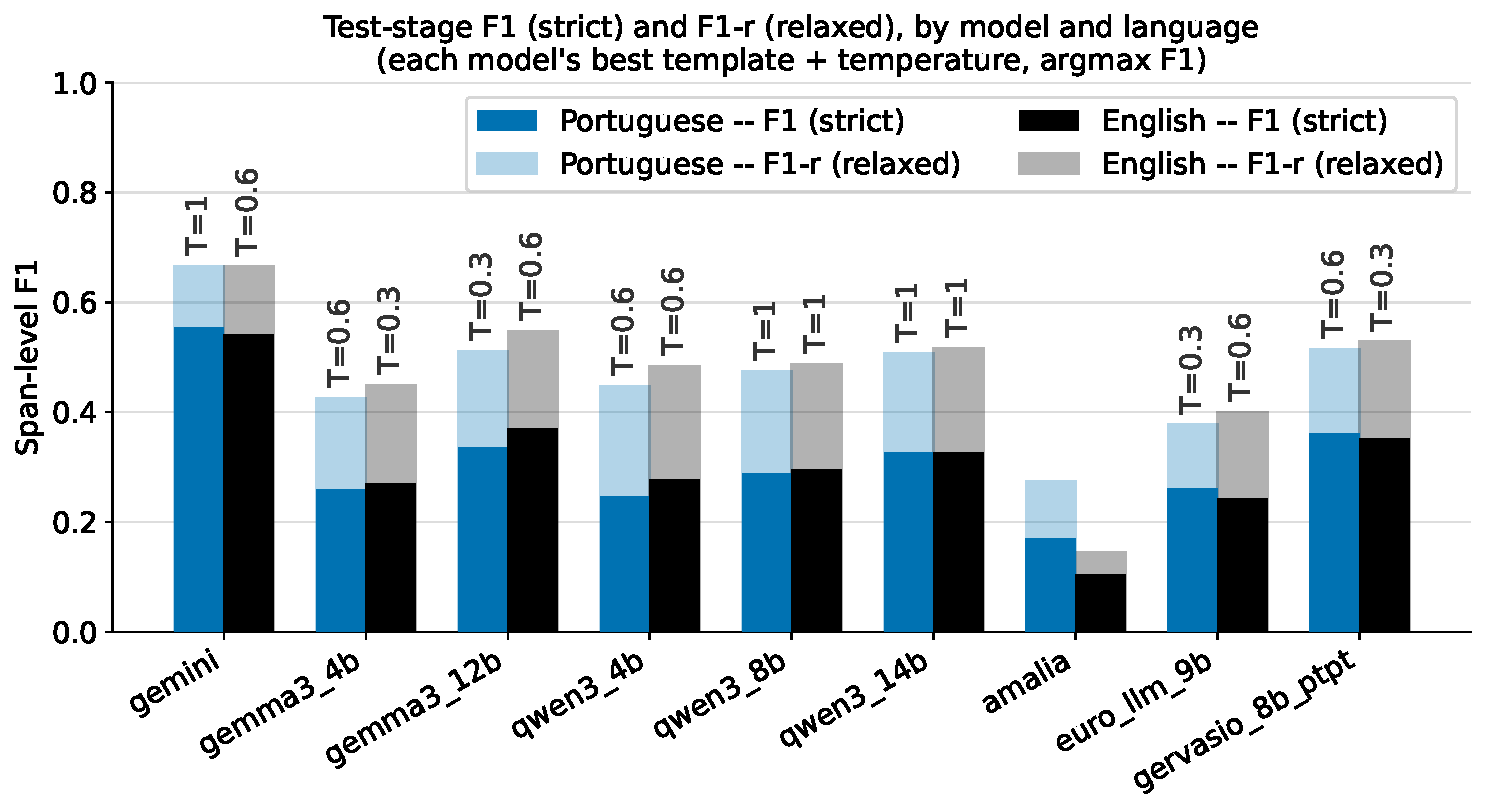
\includegraphics[width=0.80\linewidth,trim=0 0 0 50,clip]{figures/02_f1_f1r_leaderboard.pdf}
\caption{Strict F1-ext and relaxed F1-r in the test phase, by model and language, each at its best configuration. Solid fill F1-ext, full height F1-r.}
\label{fig:leaderboard}
\end{figure}

Of the 8015 document-level answers, 98.0\% were parsed. Abstentions accounted for 1.8\%, concentrated in \texttt{amalia}, which refused articles on sensitive topics such as crime and murder. Figure~\ref{fig:leaderboard} gives the resulting picture over the test partition. The baseline \texttt{gemini} leads both criteria in both languages and no open model reaches it. Except for \texttt{amalia}, each model scores similarly in both languages and the ranking is largely unchanged, indicating that performance is determined more by the model than by the language. F1-r exceeds F1-ext by a similar margin in both languages, suggesting that the models make comparable span-boundary errors.

The prompt governs span extraction far more than the language or the temperature does. Over the nine models, the median selection-phase F1-ext rises from 0.078 (bare \texttt{ext}) to 0.226 (\texttt{cls\ubk{}def\ubk{}exp}) in Portuguese and from 0.080 to 0.292 in English; the four variants carrying the one-shot example occupy the four highest ranks in both languages and the four without it the four lowest, without exception. The gain is in recall: the example does not sharpen the predictions a model already makes but leads it to extract more of the annotated participants. The definition is the weaker component, the two leading variants standing at 0.226 and 0.222 (PT) and 0.292 and 0.268 (EN). Prompt sensitivity varies more between models than between languages: for each model the standard deviation of F1-ext across the eight variants is similar in both languages, but differs substantially across models. Attribute typing is more stable, above 0.70 across the four \texttt{cls\ubk{}*} variants in both languages wherever predictions allow comparison.

\begin{table}[H]
\centering
\captionsetup{position=bottom}
{\scriptsize
\setlength{\tabcolsep}{3pt}
\begin{tabular}{@{}l rrrr@{}}
\toprule
\textbf{Model} & \textbf{F1-ext} & \textbf{Loc.} & \textbf{Typed} & \textbf{Acc.} \\
\midrule
\multicolumn{5}{@{}l}{\textbf{Portuguese} (2580 annotated participants)} \\
\texttt{gemini}             & 0.553 & 1434 & 1279 & 0.892 \\
\texttt{gemma3\ubk{}4b}     & 0.258 & 542  & 446  & 0.823 \\
\texttt{gemma3\ubk{}12b}    & 0.335 & 772  & 640  & 0.829 \\
\texttt{qwen3\ubk{}4b}      & 0.246 & 554  & 464  & 0.838 \\
\texttt{amalia}             & 0.169 & 361  & 285  & 0.789 \\
\texttt{euro\ubk{}llm\ubk{}9b} & 0.260 & 565 & 433 & 0.766 \\
\texttt{qwen3\ubk{}14b} (sent.) & 0.451 & 1031 & 927 & 0.899 \\
\addlinespace
\multicolumn{5}{@{}l}{\textbf{English} (2580 annotated participants)} \\
\texttt{gemini}             & 0.542 & 1414 & 1224 & 0.866 \\
\texttt{gemma3\ubk{}4b}     & 0.270 & 576  & 479  & 0.832 \\
\texttt{gemma3\ubk{}12b}    & 0.370 & 875  & 718  & 0.821 \\
\texttt{qwen3\ubk{}4b}      & 0.277 & 719  & 575  & 0.800 \\
\texttt{amalia}             & 0.105 & 195  & 148  & 0.759 \\
\texttt{euro\ubk{}llm\ubk{}9b} & 0.242 & 591 & 412 & 0.697 \\
\texttt{qwen3\ubk{}14b} (sent.) & 0.430 & 999 & 883 & 0.884 \\
\bottomrule
\end{tabular}}
\caption{Type-returning runs. \textbf{Loc.}: exact span matches; \textbf{Typed}: correctly typed; \textbf{Acc.}: Typed/Loc. Sentence-level runs (sent.) use $T=0.3$, others document-level; only models whose selected prompt is \texttt{cls\_*} appear.}
\label{tab:funnel}
\end{table}

Table~\ref{tab:funnel} follows the annotated participants through the two stages and locates the ceiling. Across all runs, more participants are missed at span identification than are mistyped after being located: the strongest run identifies 1434 of the 2580 annotated Portuguese participants and types 1279 of them correctly, the weakest 195 English participants and 148. The sentence-level regime confirms this by recording each stage: detection retains 84.9\%--93.5\% of sentences containing an annotated participant and classification types 86.2\%--89.9\% of the spans it receives, while extraction recovers fewer than half of the participants passed to it. Typing also varies across semantic types: overall accuracy is driven by the frequent ones, and models other than the baseline rarely assign \texttt{Nat} or \texttt{Other}.

Analysis of partial matches helps explain the gap between F1-ext and F1-r: the main extraction errors are similar across languages and concentrate on the first word of a participant span. Figure~\ref{fig:wordpos2} illustrates this pattern for two-word participants not recovered exactly, which account for about 40\% of partial matches. Their first-word match rates are 14\% (PT) and 30\% (EN), compared with 68\% and 61\%, respectively, for the second word; articles and determiners account for 75\% (PT) and 63\% (EN) of first-word errors. The same pattern persists for three- to five-word participants across document- and sentence-level runs, with first-word match rates of 12\%--20\% (PT) and 16\%--30\% (EN). The models thus identify the correct entity but disagree on whether its leading determiner belongs to the span. Cross-lingual assistance therefore offers little benefit, and neither language is consistently better: \texttt{gemma3\ubk{}12b} (0.370 vs. 0.335) and \texttt{qwen3\ubk{}4b} (0.277 vs. 0.246) favour English, \texttt{euro\ubk{}llm\ubk{}9b} (0.260 vs. 0.242) and \texttt{amalia} (0.169 vs. 0.105) Portuguese, differences no larger than between two temperatures of the same model. Input granularity matters more: on the same documents, evaluator and temperature, \texttt{qwen3\ubk{}14b} improves from 0.313 to 0.451 (PT) and 0.312 to 0.430 (EN) at sentence level (Table~\ref{tab:funnel}).

\begin{figure}[!h]
\centering
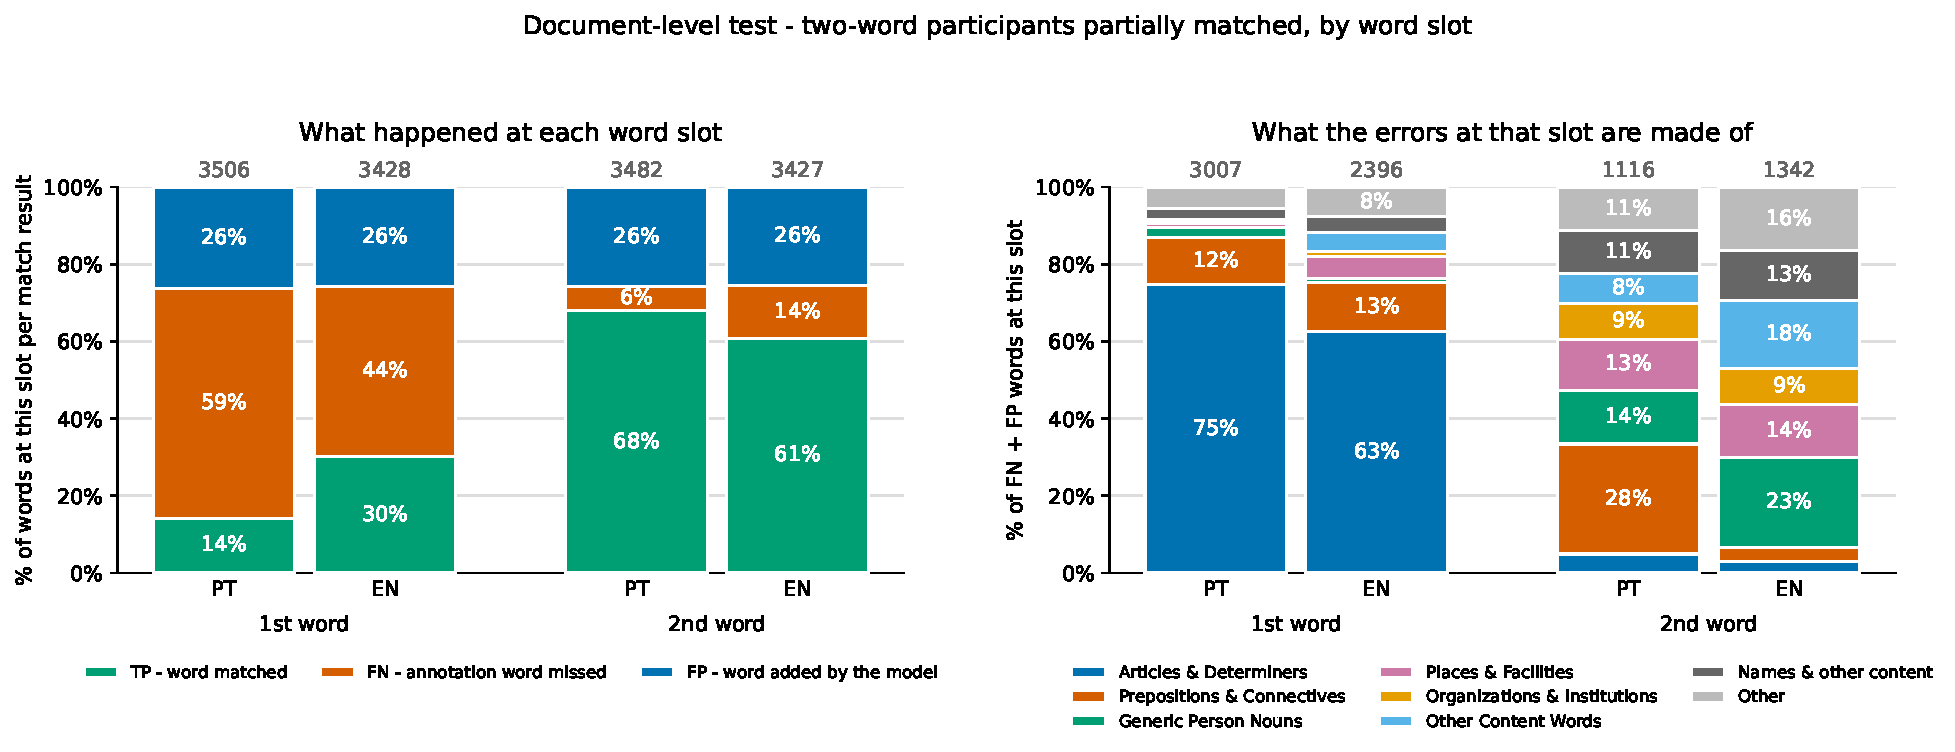
\includegraphics[width=0.70\linewidth,trim=0 0 480 40,clip]{figures/09_word_position_len2_test.pdf}
\caption{Word-level outcomes for two-word participants in the document-level test phase, pooled over models and restricted to the partial matches. The figure above a bar is the number of words it summarises.}
\label{fig:wordpos2}
\end{figure}

%-------------------------------------------------------------------------
\FloatBarrier
\section{Final Remarks and Next Steps}
\label{sec:conclusions}
\balance

The ceiling of the joint task sits at span identification rather than attribute assignment: typing accuracy stays above 0.69 wherever a span is recovered, while the strongest run recovers 1434 of the 2580 annotated participants. Prompt composition and query granularity govern that recovery and the language does not, when comparing Portuguese with English. The one-shot example and single-sentence input each moving strict extraction further than any temperature or language version does. The errors are shared between the languages and sit overwhelmingly on the determiner heading a participant, placing the limitation in the method rather than in the language. Future work should therefore target the boundary error directly, since recovering the leading determiner converts a near miss into an exact match, and extend the sentence-level decomposition beyond the single model tested here across model families.

% %-------------------------------------------------------------------------
\textbf{Acknowledgments}. This work was supported by FCT I.P. under Project
2026.00026.AIVLAB.DEUCALION – DOI – at Deucalion
supercomputer, jointly funded by EuroHPC JU and Portugal.
% This work uses the Lusa Annotated Dataset produced within the Text2Story project, and was supported by .

{\scriptsize
\bibliography{refs}
}

\end{document}
